\documentclass[12pt]{article}

\usepackage{amsmath}
\usepackage{amssymb}
\usepackage{units}
\usepackage{float}
\usepackage{graphicx}
\usepackage{amsfonts}
\usepackage{mathrsfs}
\usepackage[colorlinks]{hyperref}
\usepackage{framed}

\newcommand{\R}{\ensuremath{\mathbb{R}}}
\newcommand{\cl}[1]{\ensuremath{\mathcal{#1}}}
\newcommand{\vect}[1]{\ensuremath{\mathbf{#1}}}
\newcommand{\matr}[1]{\ensuremath{\mathbf{#1}}}
\newcommand{\mat}[2]{\left(\begin{array}{#1}#2\end{array}\right)}
\newcommand{\brc}[2]{\left\{\begin{array}{#1}#2\end{array}\right.}

\providecommand\Laplacian{\nabla^2}
\providecommand\bnabla{\boldsymbol{\nabla}}
\providecommand\bLaplacian{\boldsymbol{\nabla}^2}
\providecommand\bV{\boldsymbol{V}}
\providecommand\bx{\boldsymbol{x}}
\providecommand\bz{\boldsymbol{z}}
\providecommand\br{\boldsymbol{r}}
\providecommand\bzhat{\hat{\boldsymbol{z}}}
\providecommand\bnhat{\hat{\boldsymbol{n}}}
\providecommand\btheta{\boldsymbol{\theta}}
\providecommand\bphi{\boldsymbol{\phi}}
\providecommand\bzero{\boldsymbol{0}}

\setlength{\textheight}{8.7in}
\setlength{\columnsep}{2.0pc}
\setlength{\textwidth}{6.6in}
\setlength{\topmargin}{0.05in}
\setlength{\headheight}{0.2in}
\setlength{\headsep}{0.1in}
\setlength{\evensidemargin}{0in}
\setlength{\oddsidemargin}{0in}
\setlength{\parindent}{0.0 in}
\setlength{\parskip}{0.1 in}

\title{M.Sc. Proposal: \\ \bigskip
Computational Electrokinetics}
\author{Roman Zeyde \\ \\  {\small Advisor: Prof. Irad Yavneh} }
\begin{document}
\maketitle
\section{Introduction}
Electrokinetic theory describes the dynamics of charged particles
in ionic fluids. When a particle acquires surface charge, a layer
of ions of opposite charge is attracted to the surface via
electric forces, creating a double-layer structure around the
particle (see Figure \ref{fig:EDL}). This structure, called
``Debye layer'', electrically screens the surface charge, thus
creating a potential difference between the particle and the outer
layer of the fluid bulk.
\begin{figure}[htbp]
\begin{framed}
    \begin{center}
        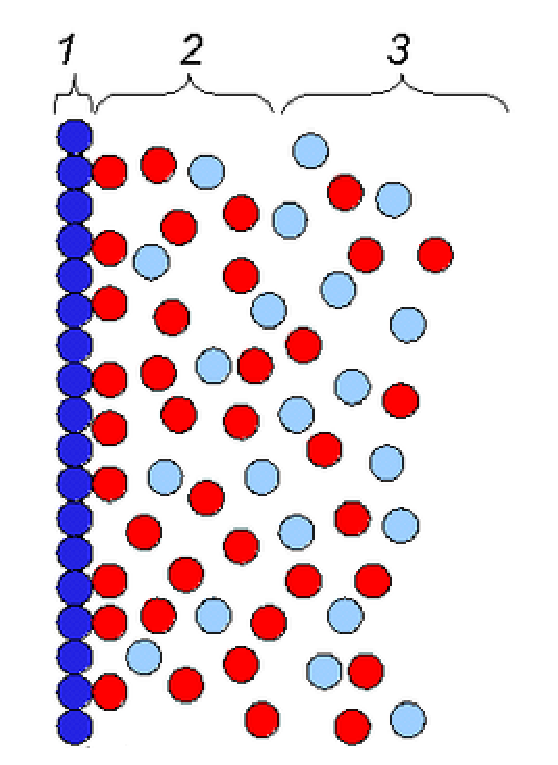
\includegraphics[width=0.25\textwidth]
            {ElectricDoubleLayer.eps}
        \caption{Schematic structure of the double layer:
        (1) particle surface, (2) Debye layer and (3) fluid bulk.
        If the particle surface has positive (blue) surface charge,
        it attracts negative (red) ions from the fluid making the
        Debye layer negatively charged (as opposed to the rest of
        the fluid bulk, which is electrically neutral).
        Zeta potential is defined as the voltage drop on (2).}
        \label{fig:EDL}
    \end{center}
\end{framed}
\end{figure}
In cases where the layer width is much smaller than the particle's
size, an analytical asymptotic solution for the Debye layer
dynamics can be found \cite{yariv2010asymptotic}.

Electrokinetics is described by the following physical phenomena (in dimensionless formulation):
\begin{enumerate}
\item Electrostatics---the fluid bulk contains no free
charge:
\begin{equation} \label{eq:Laplace}
    \bnabla \cdot (C \bnabla \varPhi) = 0 \, .
\end{equation}
\item Fluid dynamics---Stokes flow with an electrostatic force
component:
\begin{equation} \label{eq:Stokes}
\left\{ \begin{array}{l}
\bLaplacian \bV - \bnabla P + \Laplacian \varPhi \bnabla \varPhi = 0 \, , \\
\bnabla \cdot \bV = 0 \, . \end{array} \right.
\end{equation}
\item Ion diffusion and advection (via the fluid's velocity field):
\begin{equation} \label{eq:Nernst}
\Laplacian C - \alpha \bV \cdot \bnabla C = 0 \, .
\end{equation}
\end{enumerate}
The variables of the electrokinetic problem are the electrostatic
potential $\varPhi$, fluid velocity $\bV$ and its pressure $P$ and
ionic concentration $C$.

The boundary conditions are determined by the specific
problem under consideration and defined by the particle's
geometry, chemical characteristics, and the fluid dynamics.

The partial differential equations above are coupled and
non-linear. In general, they have no analytic solution. Moreover,
any numerical solver must handle the scale disparity caused by the
Debye layer width being much smaller than the particle's size. A
closed-form linear asymptotic solution has been developed for
spherical ion-exchanging particles and weak electric field in an
axisymmetric setting \cite{yariv2010migration} but it is hard to extend this
analytic solution to more general systems. Once the electric field
becomes stronger, significant nonlinear phenomena are expected.
This interesting regime has not yet been explored.

Recently, it has been conceived that such type of dynamics
can be very useful in transporting and manipulating micro-
and nanoscale objects for many nanotechnology applications,
such as the self-assembly of superstructures, roving sensors, 
drug-delivery systems and useful nanomachinery 
\cite{pumera2010electrochemically}.
However, since the analytic model for these electrokinetic
phenomena has no closed-form analytic solution, a numerical
solver has to be developed.

\section{Research goals}
Our goal is to implement an accurate and fast iterative numerical
solver for electrokinetic problems, and then apply it to the study
of systems that have no closed-form solutions, including strong
electric fields, non-spherical particles, and asymmetric charge
distribution on the particle surface. We expect to thus gain insight
into the chemical and physical behavior in far more general regimes
than are currently well-understood. We hope that this will also lead
to further analytical developments, based on new scaling behavior
provided by the numerical solver. We may also target interesting
phenomena that have been observed experimentally, e.g.,
electrophoretic\footnote{Electrophoresis is the physical
phenomenon of the motion of particles in an ion-containing fluid
under the influence of an electric field.} autonomous
micro-swimmers \cite{paxton2004catalytic, howse2007self}.

The solver will be verified against known closed-form solutions
for each of the sub-problems listed above, as well as the full
coupled problem, analyzing the discrepancies between the
theoretical (asymptotic) and numerical results. Moreover, the
convergence rate of the solver will be optimized using numerical
acceleration methods in order to achieve high accuracy in
reasonable execution time.


\section{Preliminary results}
The numerical solver is being implemented as a MATLAB package,
which provides the needed tools for numerical solution of
electrokinetic problems. The solver applies an iterative
relaxation technique to solve the discretized coupled system.
Beginning with some initial guess for the solution, the equations
are relaxed in order with respect to their corresponding
variables, with the remaining variables fixed at their current
values (``Gauss-Seidel style''):
\begin{itemize}
  \item The diffusion equation (\ref{eq:Laplace}) is used to update $\varPhi$.
  \item The Stokes system (\ref{eq:Stokes}) is used to update $\bV$ and $P$.
  \item The Nernst-Planck equation (\ref{eq:Nernst}) is used to update $C$.
\end{itemize}

The problem configuration is taken from \cite{yariv2010migration} and
consists of a spherical ion-exchanging particle, surrounded by
infinite Stokes fluid. Spherical coordinates $(R,\theta,\phi)$ are
employed. The problem is axisymmetric, hence independent of
$\phi$, which simplifies the solution process. The electrokinetic
problem is thus written as a two-dimensional partial differential
equation system for $R \in [1,\infty)$ and $\theta \in [0, \pi]$.
Natural grid choices are a logarithmic grid for $R$ and a uniform
grid for $\theta$.

The following linear operators are implemented in spherical
coordinates on the grid described above: Scalar Laplacian (for
$\varPhi$ and $C$), Vector Laplacian (for $\bV$), Gradient (for
$\Phi, C$ and $P$) and Divergence (for $\bV$). Each differential
operator is written in spherical coordinates on the regular $(R,
\theta)$ grid and, being linear, is represented as a sparse
matrix, which is very convenient for the required algebraic
manipulations.

The boundary conditions are defined for $\theta = 0$ and $\theta =
\pi$ using symmetry considerations. At $R = \infty$, we assume
constant fluid velocity $\bV = \cl{U} \bzhat$, constant electric
field $\bnabla \varPhi = -\beta \bzhat$ and constant ionic
concentration $C = 1$. The boundary conditions on $R = 1$ are
defined by the Debye layer's behavior as described in
\cite{yariv2010migration}, using the Dukhin-�Derjaguin slip formula for
$\bV$ and ion-selectivity for $\varPhi$ and $C$.

Each differential equation and its boundary conditions are
discretized, resulting in a sparse linear system of the form
$\matr{A}\bx = \vect{b}$. We then cycle by applying a few
relaxation iterations on each linear system in turn, as noted
above, using an appropriate preconditioner
$\matr{M}_\matr{A}^{-1}$:
\begin{eqnarray} \label{eq:Relax}
  \bx_{n+1} &=& \bx_{n} + \matr{M}_\matr{A}^{-1} \left(\vect{b} - \matr{A}\bx_{n}\right)
\end{eqnarray}

After the iterations have converged to a solution for the coupled
system, the total stress tensor $\mathbb{T}$ on the particle
$\cl{S} = \left\{\bx : \|\bx\| = 1\right\}$ is computed
(\ref{eq:Stress}) and integrated to yield the total force
(\ref{eq:Force}):
\begin{eqnarray}
  \label{eq:Stress}
  \mathbb{T} &=& - P \mathbb{I} + \bnabla \bV + (\bnabla \bV) ^T  +
  \bnabla \varPhi \bnabla \varPhi - \frac{\bnabla \varPhi \cdot \bnabla \varPhi}{2} \mathbb{I}, \\
  \label{eq:Force}
  \vect{F} &=& \int_{\cl{S}} \left(\mathbb{T} \cdot \bnhat \right) ds = \boldsymbol{0}.
\end{eqnarray}
Because the problem is axisymmetric, the force should be aligned
with the symmetry axis: $\vect{F} = F \bzhat$. Moreover, since the
particle is stress-free in steady flow, we have $F = 0$ for
steady-state velocity $\cl{U}$. This observation enables us to
find the correct $\cl{U}$ for given $\beta$, using a
one-dimensional root-finding algorithm on $F_\beta(\cl{U})$, as a
function of $\cl{U}$.

The numerical solution for $\cl{U}$ as a function of $\beta$ is
compared to the closed-form asymptotic solution from
\cite{yariv2010migration}. Using a $60 \times 15$ grid for $(R,\theta) \in
[1, 100] \times [0, \pi]$, we apply $2\mathord{,}000$ iterations
in order to find the total force acting on the particle. This step
is repeated a few times to find the correct $\cl{U}$ so that
$F_\beta(\cl{U}) = 0$ for various $\beta$ values---see Figure
\ref{fig:Results} for numerical results.
\begin{figure}[htbp]
\begin{framed}
    \begin{center}
        \includegraphics[width=0.45\textwidth]
            {convergence.eps}
        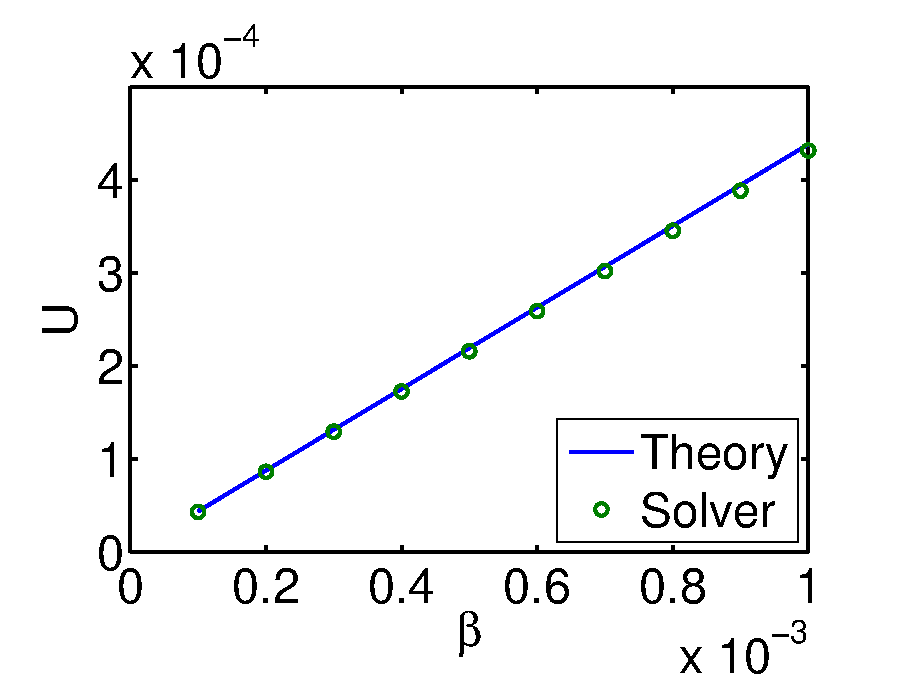
\includegraphics[width=0.45\textwidth]
            {comparison.eps}
        \caption{Left: Residual $\ell_2$ norm convergence graph. Right: Particle Velocity
        $\cl{U}$ as a the function of electric field $\beta$.
        The error between the theoretical and the solver's results is less than 2\%.}
        \label{fig:Results}
    \end{center}
\end{framed}
\end{figure}

\section{Algorithms and techniques}

$C$, $\varPhi$ and $P$ are discretized at cell centers, whereas a
staggered grid is used for $\bV$ at the problem domain $\cl{D}$
(see Figure \ref{fig:Grids}).
\begin{figure}[htbp]
\begin{framed}
    \begin{center}
        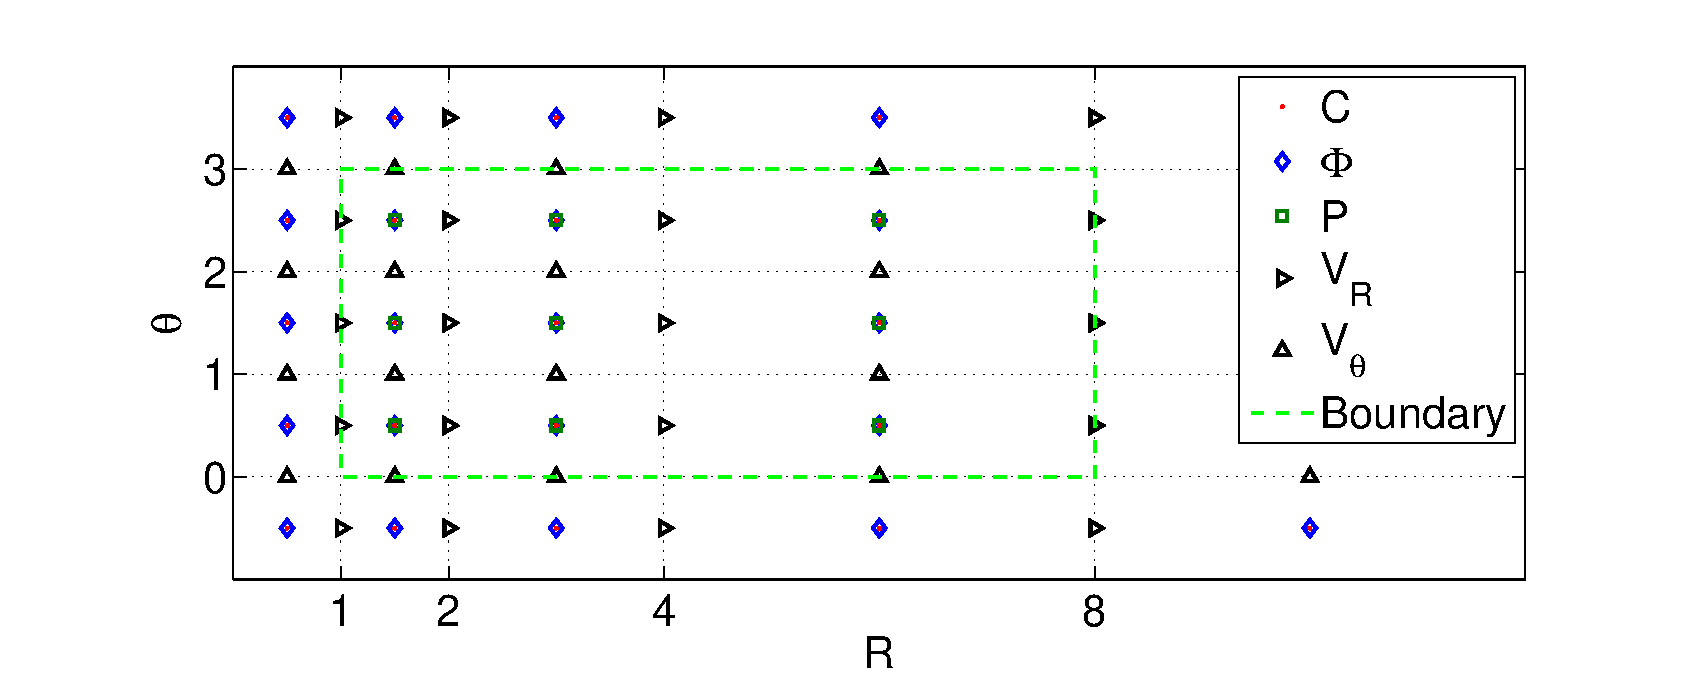
\includegraphics[width=1\textwidth]
            {StaggeredGrid.eps}
        \caption{Grids for $C$, $\varPhi$, $P$ and $\bV$.}
        \label{fig:Grids}
    \end{center}
\end{framed}
\end{figure}
A finite volume discretization is used to represent the partial
differential equations in the form of an algebraic system, using
central differences or an upwind scheme (for stability). ``Ghost
points'' are used to define Dirichlet and Neumann boundary
conditions on the domain boundary $\partial \cl{D}$.

After boundary conditions are eliminated, Jacobi and Red-Black
Gauss-Seidel preconditioners are used for equations
(\ref{eq:Laplace}) and (\ref{eq:Nernst}), while a so-called
Vanka-type \cite{vanka1986block} preconditioner is used for equation
(\ref{eq:Stokes}). The preconditioners are computed as sparse
matrices, facilitating the relaxation process (\ref{eq:Relax}).

Vector extrapolation methods \cite{sidi1991efficient} have been 
implemented and are used to accelerate the solver's convergence. 
Later, a Multigrid framework \cite{brandt1977multi, yavneh2006multigrid} 
will be introduced to allow the efficient solution of large problems.

\bibliographystyle{plain}
\bibliography{proposal}

\end{document}
